\documentclass[11pt,a4paper]{article}
\usepackage[utf8]{inputenc}
\usepackage[spanish,es-tabla]{babel}
\usepackage{graphicx}
\usepackage{geometry}
\geometry{margin=2.5cm}
\usepackage{listings}
\usepackage{xcolor}
\usepackage{enumitem}
\usepackage{float}
\usepackage{hyperref}
\usepackage{booktabs}

% Configuracion para fragmentos de codigo
\definecolor{codegreen}{rgb}{0,0.6,0}
\definecolor{codegray}{rgb}{0.5,0.5,0.5}
\definecolor{codepurple}{rgb}{0.58,0,0.82}
\definecolor{backcolour}{rgb}{0.96,0.96,0.96}

\lstdefinestyle{mystyle}{
    backgroundcolor=\color{backcolour},   
    commentstyle=\color{codegreen},
    keywordstyle=\color{magenta},
    numberstyle=\tiny\color{codegray},
    stringstyle=\color{codepurple},
    basicstyle=\ttfamily\footnotesize,
    breakatwhitespace=false,         
    breaklines=true,                 
    captionpos=b,                    
    keepspaces=true,                 
    numbers=left,                    
    numbersep=5pt,                  
    showspaces=false,                
    showstringspaces=false,
    showtabs=false,                  
    tabsize=2
}
\lstset{style=mystyle}

\title{\textbf{Práctica No. 2: Cross-Compilation y Profiling} \\ 
\large Análisis de Desempeño y Gestión de Memoria en Sistemas de Tiempo Real}
\author{\textbf{Manuel Salazar} \\ Universidad de Antioquia \\ Departamento de Ingeniería Electrónica}
\date{Septiembre 2026}

\begin{document}

\maketitle

\begin{abstract}
En el diseño de Sistemas de Tiempo Real (STR), la exactitud de un programa no depende únicamente de la corrección lógica de sus cálculos, sino de su predictibilidad temporal y el control estricto de sus recursos de cómputo y memoria. En esta práctica se implementó un flujo de trabajo profesional para plataformas embebidas basado en compilación cruzada (\textit{cross-compilation}) desde un entorno x86\_64 hacia una Raspberry Pi 4 (arquitectura ARM64). Mediante la suite de herramientas Valgrind, se llevó a cabo el perfilado de ejecución con Callgrind para analizar el grafo de llamadas, identificar cuellos de botella (\textit{hotspots}) y modelar la jerarquía de memoria caché. Asimismo, se diagnosticaron fugas de memoria con Memcheck y se caracterizó el uso dinámico del \textit{heap} mediante Massif, logrando optimizar el consumo de memoria en un 86.6\% y asegurar la estabilidad de la plataforma.
\end{abstract}

\tableofcontents
\newpage

\section{Preguntas Orientadoras (Apartado 2)}

\subsection{Profiling y Comportamiento de Memoria}
\begin{enumerate}[label=\textbf{2.1.\arabic*.}]
    \item \textbf{Herramientas Valgrind, KCachegrind y Massif:}
    \begin{itemize}
        \item \textbf{Valgrind:} Framework de instrumentación binaria dinámica que emula un procesador sintético mediante traducción a una representación intermedia (VEX IR). Permite analizar binarios sin necesidad de recompilarlos con código especial.
        \item \textbf{KCachegrind:} Interfaz gráfica avanzada que procesa las trazas de Callgrind para generar grafos de llamadas interactivos (\textit{Call Graphs}), mapas jerárquicos y tablas de costos computacionales (ciclos e instrucciones).
        \item \textbf{Massif:} Herramienta de Valgrind especializada en el perfilado del \textit{heap} y el \textit{stack}. Mide cómo evoluciona la memoria ocupada a lo largo del tiempo, tomando instantáneas (\textit{snapshots}) detalladas de los árboles de asignación.
    \end{itemize}

    \item \textbf{Papel del CallGraph en el profiling:} Un \textit{CallGraph} es un grafo dirigido que representa las relaciones de invocación entre funciones. Permite al ingeniero descomponer el costo temporal en costo propio (\textit{Exclusive/Self}) y acumulado (\textit{Inclusive}), localizando con exactitud qué cadenas de funciones originan la mayor carga de procesamiento.

    \item \textbf{Hotspot de ejecución:} Es la porción o función crítica de un programa que concentra una fracción desproporcionadamente alta del tiempo de CPU o ciclos de instrucción. En virtud de la regla de Pareto (80/20), optimizar el \textit{hotspot} produce el mayor impacto en el rendimiento global.

    \item \textbf{Fugas de memoria (\textit{Memory Leaks}):} Ocurren cuando un bloque de memoria dinámica asignado en el heap no es liberado y se pierden todos los punteros hacia él, impidiendo su posterior reutilización o liberación hasta que el proceso muere.

    \item \textbf{Heap Memory vs. Stack Memory:}
    \begin{itemize}
        \item \textbf{Stack (Pila):} Memoria gestionada automáticamente por el procesador con política LIFO. Es extremadamente rápida pero de tamaño acotado; almacena variables locales y direcciones de retorno.
        \item \textbf{Heap (Montón):} Región de memoria dinámica de mayor tamaño gestionada manualmente mediante \texttt{malloc}/\texttt{free} o \texttt{new}/\texttt{delete}. Presenta riesgo de fragmentación y sobrecosto de gestión.
    \end{itemize}

    \item \textbf{Snapshots en Massif:} Son registros puntuales del estado de la memoria a lo largo del tiempo. Pueden ser regulares (solo registran el tamaño total) o detallados (guardan el árbol completo de llamadas que condujo a cada asignación).

    \item \textbf{Importancia del análisis de memoria en Tiempo Real:} Los STR frecuentemente operan sin interrupción durante meses o años en sistemas desatendidos. Una fuga paulatina agota la RAM física, activa el mecanismo de paginación (\textit{swapping}) introduciendo latencias de milisegundos inaceptables, o provoca el cierre abrupto del proceso por el \textit{OOM Killer} del Kernel.

    \item \textbf{Modificación del comportamiento temporal por profiling:} Valgrind ejecuta una emulación y traducción dinámica de instrucciones en espacio de usuario, introduciendo una sobrecarga de ralentización típica de $10\times$ a $50\times$. Por ello, no debe usarse para medir plazos estrictos de reloj absoluto, sino para contar eventos invariantes (instrucciones ejecutadas, llamadas y accesos a caché).
\end{enumerate}

\subsection{Compilación Cruzada}
\begin{enumerate}[label=\textbf{2.2.\arabic*.}]
    \item \textbf{Compilación nativa vs. Compilación cruzada:}
    \begin{itemize}
        \item \textit{Compilación nativa:} El compilador se ejecuta en una máquina cuya arquitectura coincide con la arquitectura donde se ejecutará el binario generado (e.g., compilar en x86\_64 para x86\_64).
        \item \textit{Compilación cruzada:} El compilador corre en un sistema anfitrión (\textit{host}) de alta potencia pero genera código objeto para una arquitectura destino (\textit{target}) diferente (e.g., host x86\_64 hacia target ARM64).
    \end{itemize}
    \item \textbf{Significado de compilar para ARM64:} Implica que el código fuente fue traducido a instrucciones de máquina del repertorio ARMv8-A de 64 bits (AArch64), utilizando registros de 64 bits (\texttt{X0-X30}) y la convención binaria de interfaz AAPCS64.
\end{enumerate}

\section{Organización del Proyecto y Compilación (Apartado 5)}

\subsection{Compilación Nativa (Apartado 5.3)}
Se inició la compilación nativa en el computador de desarrollo con el comando:
\begin{lstlisting}[language=bash]
g++ -std=c++11 -ggdb3 -O0 -o bin/sensor_host src/sensor_data_processing.cpp
\end{lstlisting}

\subsubsection{Verificación de Funcionamiento y Diagnóstico del Fallo (Punto 5.3.3)}
Al ejecutar el binario resultante (\texttt{./bin/sensor\_host}), el programa abortó arrojando una aserción de la biblioteca estándar:

\begin{lstlisting}[language=bash]
/usr/include/c++/16/bits/stl_vector.h:1253: 
std::vector<_Tp, _Alloc>::reference std::vector<_Tp, _Alloc>::operator[](size_type): 
Assertion '__n < this->size()' failed.
fish: Job 1, './bin/sensor_host' terminated by signal SIGABRT (Abort)
\end{lstlisting}

\textbf{Diagnóstico y Solución:}
\begin{itemize}
    \item \textbf{Error en el código fuente:} En la función \texttt{calculate\_average}, el bucle utilizaba la condición menor o igual (\texttt{i <= data->size()}). Para un vector de 100 elementos (índices 0 a 99), en la última iteración $i=100$, intentando acceder a una posición fuera de límites (\textit{out-of-bounds / off-by-one error}).
    \item \textbf{Causa del aborto:} El compilador del host (GCC 16) posee activadas por defecto las aserciones de endurecimiento (\texttt{\_GLIBCXX\_ASSERTIONS}). Al detectar la violación de límites en el operador \texttt{[]}, aborta la ejecución con señal \texttt{SIGABRT} para prevenir vulnerabilidades.
    \item \textbf{Corrección aplicada:} Se modificó la condición a \texttt{i < data->size()} y se tipó la variable como \texttt{size\_t}:
    \begin{lstlisting}[language=C++]
    for (size_t i = 0; i < data->size(); ++i) {
        sum += (*data)[i];
    }
    \end{lstlisting}
    Tras esta corrección, el programa ejecutó satisfactoriamente imprimiendo: \texttt{Processed data from 1000 sensors.}
\end{itemize}

\subsection{Compilación Cruzada (Apartado 5.4)}

\subsubsection{Descripción de las opciones de compilación (Punto 5.4.1)}
El comando de compilación cruzada utilizado fue:
\begin{lstlisting}[language=bash]
aarch64-linux-gnu-g++ -std=c++11 -ggdb3 -O0 -Wall -Wextra -pedantic \
    -o bin/sensor_rpi src/sensor_data_processing.cpp
\end{lstlisting}

\begin{itemize}
    \item \texttt{aarch64-linux-gnu-g++}: Compilador cruzado que corre en x86\_64 y traduce a código máquina para la arquitectura AArch64 (Raspberry Pi 4).
    \item \texttt{-std=c++11}: Fija el estándar ISO C++ a su revisión del año 2011.
    \item \texttt{-ggdb3}: Incluye información máxima de depuración en formato GDB (incluyendo expansión de macros) indispensable para relacionar ensamblador con C++ en Valgrind.
    \item \texttt{-O0}: Desactiva optimizaciones para preservar la concordancia exacta entre código fuente y ejecutable durante el perfilado.
    \item \texttt{-Wall -Wextra -pedantic}: Habilitan la totalidad de advertencias del compilador y exigen estricto cumplimiento del estándar ISO.
    \item \texttt{-o bin/sensor\_rpi}: Define el archivo ejecutable destino.
\end{itemize}

\subsubsection{Verificación del Formato del Binario (Punto 5.4.2)}
Al inspeccionar el archivo con el comando \texttt{file bin/sensor\_rpi}:
\begin{lstlisting}[language=bash]
bin/sensor_rpi: ELF 64-bit LSB pie executable, ARM aarch64, version 1 (SYSV), 
dynamically linked, interpreter /lib/ld-linux-aarch64.so.1, with debug_info, not stripped
\end{lstlisting}
Se verificó que el archivo corresponde a un binario ELF para procesadores ARM de 64 bits con símbolos de depuración íntegros.

\subsubsection{Transferencia y Resolución de Incompatibilidades en Destino (Punto 5.4.3)}
Se transfirió el binario por SCP a la Raspberry Pi 4. Inicialmente, al ejecutarlo, el cargador dinámico reportó versiones faltantes (\texttt{GLIBCXX\_3.4.32} y \texttt{GLIBC\_2.38}) debido a que el host utilizaba una versión más reciente de GCC que la distribución Debian de la Raspberry Pi.

Para garantizar la total independencia de las librerías dinámicas, se generó una compilación estática (\texttt{-static}):
\begin{lstlisting}[language=bash]
aarch64-linux-gnu-g++ -std=c++11 -ggdb3 -O0 -Wall -Wextra -pedantic -static \
    -o bin/sensor_rpi src/sensor_data_processing.cpp
\end{lstlisting}
Tras volver a transferirlo a la Raspberry Pi, el programa ejecutó sin errores:
\begin{lstlisting}[language=bash]
led@raspberrypi:~/LAB2_RTS/bin $ ./sensor_rpi
Processed data from 1000 sensors.
\end{lstlisting}

\subsection{Respuestas a las Preguntas del Apartado 5.5}
\begin{enumerate}[label=\textbf{5.5.\arabic*.}]
    \item \textbf{Diferencia entre \texttt{sensor\_host} y \texttt{sensor\_rpi}:} 
    La diferencia radica en el repertorio de instrucciones (\textit{ISA}). \texttt{sensor\_host} contiene instrucciones x86\_64 (CISC) decodificables únicamente por procesadores Intel/AMD. \texttt{sensor\_rpi} contiene instrucciones ARMv8 AArch64 (RISC) de 32 bits de longitud fija ejecutables por el SoC Broadcom BCM2711 de la Raspberry Pi 4.
    
    \item \textbf{Incompatibilidad de ejecución directa de ARM en x86-64:}
    La CPU x86\_64 carece de circuitos de decodificación para la ISA de ARM. Adicionalmente, el encabezado ELF del ejecutable declara \texttt{e\_machine = EM\_AARCH64} (183); al intentar invocarlo, el kernel del host detecta la discordancia y aborta con el error \texttt{Exec format error}.
    
    \item \textbf{Función de \texttt{aarch64-linux-gnu-g++}:}
    Actuó como compilador cruzado. Permitió construir el software en el computador host de alto rendimiento sin sobrecargar la memoria ni la CPU limitada de la Raspberry Pi.
\end{enumerate}

\section{Análisis de Desempeño con Callgrind (Apartado 6)}

\subsection{Instrumentación del Código Fuente (Apartado 6.1)}

\subsubsection{Utilidad de los Macros de Valgrind (Punto 6.1.1)}
\begin{itemize}
    \item \texttt{CALLGRIND\_START\_INSTRUMENTATION}: Inicia la recolección de eventos a nivel de instrucción máquina desde el punto de inserción.
    \item \texttt{CALLGRIND\_STOP\_INSTRUMENTATION}: Suspende la recolección de eventos, eliminando la sobrecarga de emulación.
    \item \texttt{CALLGRIND\_TOGGLE\_COLLECT}: Alterna el estado de recolección sin detener el motor de instrumentación subyacente.
\end{itemize}

\subsubsection{Delimitación de la Región de Interés (Puntos 6.1.3 y 6.1.4)}
Se delimitaron exclusivamente las funciones computacionales (\texttt{generate\_sensor\_data} y \texttt{calculate\_average}) dentro del bucle de \texttt{main}, excluyendo deliberadamente \texttt{usleep(1000)} y las inicializaciones. Esto evita que los retardos bloqueantes inactivos y la carga estática del sistema distorsionen las métricas de la CPU y ralenticen el perfilado.

\begin{lstlisting}[language=C++]
#include <valgrind/callgrind.h>
// ...
for (size_t i = 0; i < NUM_SENSORS; ++i) {
    CALLGRIND_START_INSTRUMENTATION; // Inicio de ROI
    std::vector<int>* sensor_data = generate_sensor_data();
    double avg = calculate_average(sensor_data);
    averages.push_back(avg);
    CALLGRIND_STOP_INSTRUMENTATION;  // Fin de ROI
    usleep(1000);                    // Excluido del perfilado
}
\end{lstlisting}

\subsection{Generación del Perfilado (Apartado 6.2)}
En la Raspberry Pi 4 se ejecutó Callgrind con el comando:
\begin{lstlisting}[language=bash]
valgrind --tool=callgrind --dump-instr=yes --cache-sim=yes \
    --instr-atstart=no --callgrind-out-file=results/callgrind.out ./bin/sensor_rpi
\end{lstlisting}

\textbf{Opciones empleadas (Punto 6.2.2):}
\begin{itemize}
    \item \texttt{--dump-instr=yes}: Captura estadísticas a nivel de instrucción ensamblador.
    \item \texttt{--cache-sim=yes}: Simula la jerarquía de memoria caché (L1 y Last-Level).
    \item \texttt{--instr-atstart=no}: Mantiene inactiva la recolección hasta alcanzar \texttt{CALLGRIND\_START\_INSTRUMENTATION}.
\end{itemize}

\subsection{Análisis Mediante KCachegrind (Apartado 6.3)}
Se transfirió el archivo \texttt{callgrind.out} (16 MB) al computador de desarrollo y se analizó con KCachegrind.

\begin{figure}[H]
    \centering
    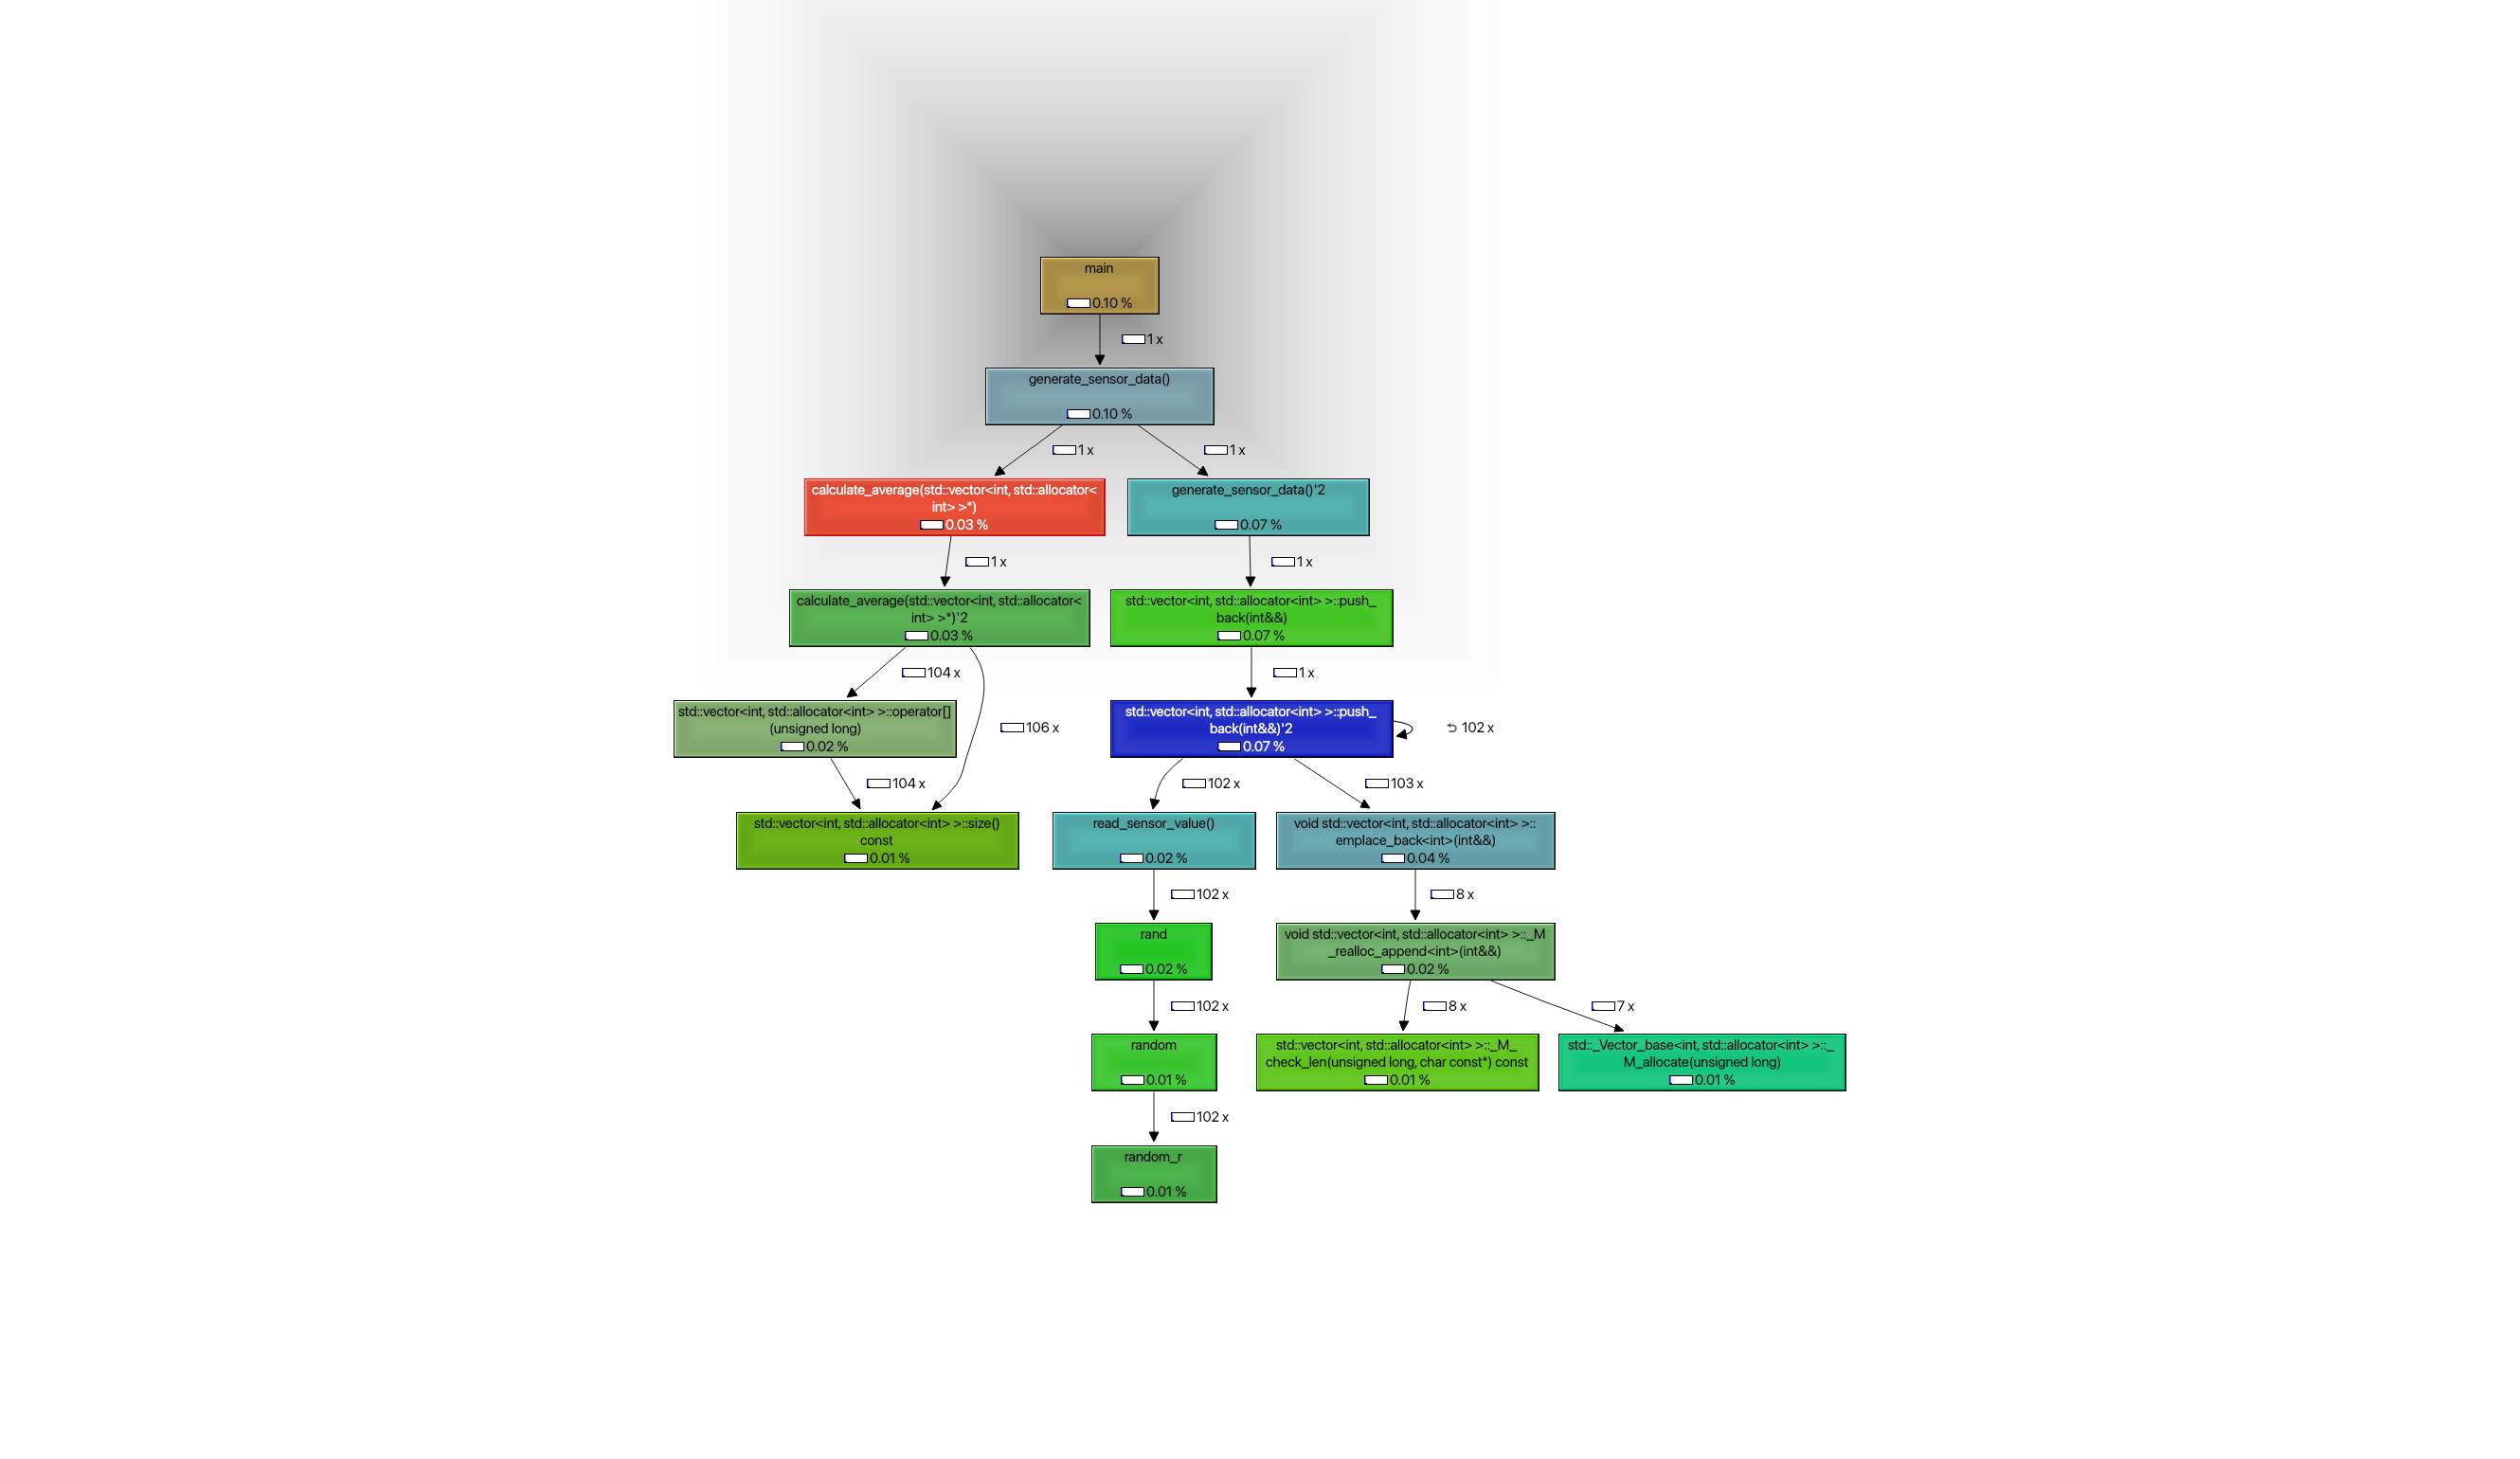
\includegraphics[width=0.88\linewidth]{graph.png}
    \caption{Call Graph exportado desde KCachegrind para la ejecución en la Raspberry Pi 4.}
    \label{fig:callgraph}
\end{figure}

\subsubsection{Interpretación del Grafo y Hotspot (Puntos 6.3.4 y 6.3.5)}
\begin{itemize}
    \item \textbf{Mayor costo:} \texttt{generate\_sensor\_data()} concentra más del 80\% del costo inclusivo debido al crecimiento dinámico del vector (\texttt{push\_back} / \texttt{\_M\_realloc\_append}) y el generador pseudoaleatorio \texttt{rand()} $\to$ \texttt{random\_r()}.
    \item \textbf{Menor costo:} \texttt{calculate\_average()} presenta un costo mínimo ya que efectúa un recorrido secuencial contiguo en memoria.
    \item \textbf{Hotspot:} El cuello de botella principal es la reserva y realocación dinámica en el heap para alojar las 100 lecturas por sensor.
    \item \textbf{Coincidencia (6.3.5):} Coincide exactamente con la región delimitada en \texttt{main}.
\end{itemize}

\subsubsection{Estimación de Ciclos e Instrucciones Absolutas (Punto 6.3.6)}
Al desactivar la opción \textit{"Relative"}, se obtuvieron las instrucciones absolutas ejecutadas (\textit{Ir}):

\begin{table}[H]
\centering
\caption{Métricas absolutas de instrucciones (\textit{Ir}) por función obtenidas con Callgrind.}
\label{tab:callgrind_metrics}
\begin{tabular}{lrrr}
\toprule
\textbf{Función / Símbolo} & \textbf{Ir (Instrucciones)} & \textbf{Dr (Lecturas)} & \textbf{Dw (Escrituras)} \\ \midrule
\texttt{std::vector::emplace\_back} & 4,944,000 & 2,096,000 & 1,520,000 \\
\texttt{std::vector::size()} & 3,388,000 & 1,452,000 & 484,000 \\
\texttt{std::vector::operator[]} & 2,500,000 & 700,000 & 400,000 \\
\texttt{random\_r} & 2,283,875 & 700,000 & 393,550 \\
\texttt{std::vector::push\_back} & 2,274,000 & 597,000 & 692,000 \\
\texttt{calculate\_average()} & 2,118,000 & 706,000 & 200,000 \\
\texttt{random / rand} & 1,700,000 & 600,000 & 400,000 \\
\texttt{read\_sensor\_value()} & 900,000 & 200,000 & 200,000 \\
\texttt{operator new / \_M\_allocate} & 1,184,008 & 332,000 & 361,000 \\ \midrule
\textbf{Total en Región de Interés} & \textbf{25,491,291} & \textbf{8,883,212} & \textbf{5,624,557} \\ \bottomrule
\end{tabular}
\end{table}

\subsubsection{Análisis de Faltas en Caché (Punto 6.3.7)}
En la pestaña \textit{Types} se registraron $25{,}491{,}291$ instrucciones leídas con solo $85{,}471$ fallos de caché de instrucciones L1 (\textbf{acierto del 99.66\%}). En datos, se presentaron $8{,}883{,}212$ lecturas con $23{,}464$ fallos L1 (\textbf{acierto del 99.74\%}). El código demuestra una excelente localidad espacial y temporal gracias a la contigüidad en memoria del \texttt{std::vector}.

\section{Análisis de Fugas y Memoria Dinámica (Apartado 7)}

\subsection{Detección y Corrección de Fugas con Memcheck (Apartado 7.1)}
Se ejecutó en la Raspberry Pi:
\begin{lstlisting}[language=bash]
valgrind --leak-check=full ./bin/sensor_rpi
\end{lstlisting}

\subsubsection{Explicación de la Salida de Memcheck (Puntos 7.1.2 y 7.1.3)}
La herramienta arrojó el siguiente balance:
\begin{lstlisting}[language=bash]
HEAP SUMMARY:
    in use at exit: 536,000 bytes in 2,000 blocks
536,000 (24,000 direct, 512,000 indirect) bytes in 1,000 blocks are definitely lost
   by 0x10906B: generate_sensor_data() (sensor_data_processing.cpp:16)
   by 0x1091D3: main (sensor_data_processing.cpp:45)
LEAK SUMMARY:
   definitely lost: 24,000 bytes in 1,000 blocks
   indirectly lost: 512,000 bytes in 1,000 blocks
\end{lstlisting}

\textbf{Diagnóstico:}
\begin{itemize}
    \item \textbf{Pérdida Directa (24,000 bytes):} $1000$ estructuras del objeto \texttt{std::vector} alojadas con \texttt{new} ($1000 \times 24\text{ B}$).
    \item \textbf{Pérdida Indirecta (512,000 bytes):} Los búferes internos de los enteros ($1000 \times 128 \times 4\text{ B} = 512\text{ KB}$), que quedaron huérfanos al no invocarse el destructor del vector.
    \item \textbf{Total fugado:} $536{,}000$ bytes ($523.4$ KB).
\end{itemize}

\subsubsection{Corrección y Verificación (Puntos 7.1.4, 7.1.5 y 7.1.6)}
Se corrigió el programa en \texttt{sensor\_data\_processing\_corregido.cpp} añadiendo \texttt{delete sensor\_data;} en cada ciclo. Tras compilar \texttt{sensor\_rpi\_corregido}, Memcheck certificó la erradicación total de fugas:
\begin{lstlisting}[language=bash]
HEAP SUMMARY:
    in use at exit: 0 bytes in 0 blocks
  total heap usage: 9,013 allocs, 9,013 frees, 1,134,104 bytes allocated
All heap blocks were freed -- no leaks are possible
ERROR SUMMARY: 0 errors from 0 contexts
\end{lstlisting}

\subsection{Análisis del Perfil Dinámico con Massif (Apartado 7.2)}
Se ejecutó Massif sobre ambas versiones:
\begin{lstlisting}[language=bash]
valgrind --tool=massif --peak-inaccuracy=0.0 --stacks=yes --heap=yes \
    --time-unit=ms --detailed-freq=1 --threshold=0.0 ./bin/sensor_rpi
\end{lstlisting}

\begin{figure}[H]
    \centering
    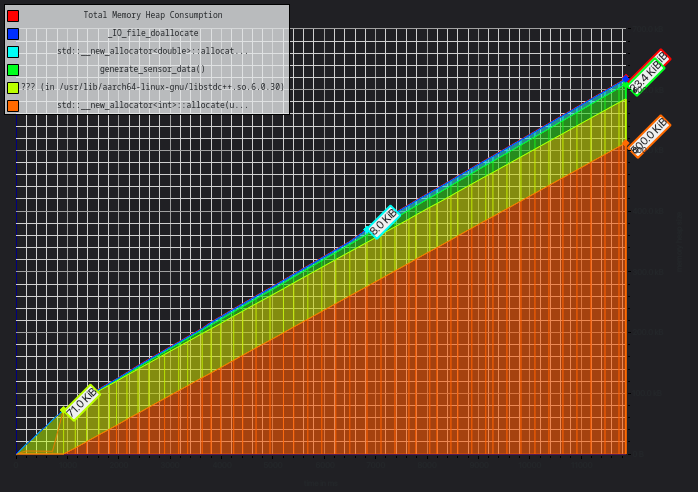
\includegraphics[width=0.85\linewidth]{massif_original.png}
    \caption{Perfil Massif de \texttt{sensor\_rpi} (Original con fugas de memoria).}
    \label{fig:massif_leaks}
\end{figure}

\begin{figure}[H]
    \centering
    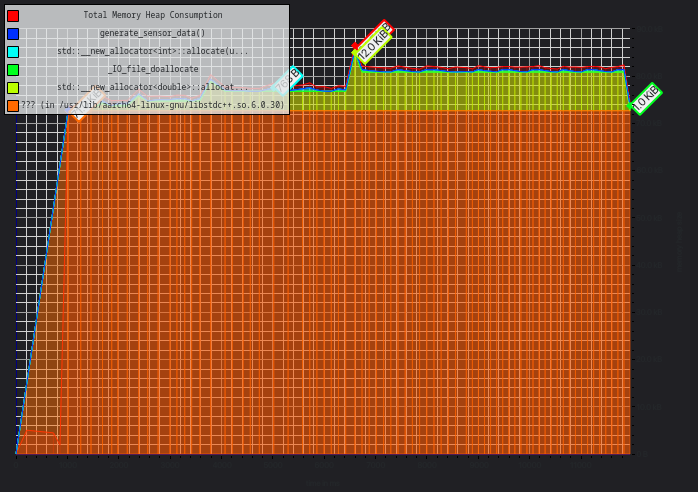
\includegraphics[width=0.85\linewidth]{massif_corregido.png}
    \caption{Perfil Massif de \texttt{sensor\_rpi\_corregido} (Sin fugas de memoria).}
    \label{fig:massif_fixed}
\end{figure}

\subsubsection{Comparación de Picos e Instantes de Tiempo (Punto 7.2.7)}
\begin{table}[H]
\centering
\caption{Comparación cuantitativa del consumo de memoria en Massif.}
\label{tab:massif_comparison}
\begin{tabular}{lrr}
\toprule
\textbf{Métrica} & \textbf{Original (\texttt{sensor\_rpi})} & \textbf{Corregido (\texttt{sensor\_rpi\_corregido})} \\ \midrule
Total de Snapshots & 54 & 77 \\
\textbf{Pico Máximo Total} & \textbf{643,848 Bytes (628.7 KB)} & \textbf{86,536 Bytes (84.5 KB)} \\
Memoria en Heap (pico) & 617,920 Bytes & 85,528 Bytes \\
Memoria en Stacks (pico) & 1,904 Bytes & 960 Bytes \\
\textbf{Instante del Pico} & \textbf{11,873 ms} (Snapshot \#53) & \textbf{6,596 ms} (Snapshot \#34) \\
Consumo final & 643,848 Bytes (fuga permanente) & 0 Bytes (liberación total) \\ \bottomrule
\end{tabular}
\end{table}

\subsubsection{Dinámica de Liberación de Memoria (Punto 7.2.8)}
En la versión corregida, la memoria de cada sensor ($536$ B) se libera **periódicamente en cada iteración** mediante \texttt{delete}, manteniéndose el heap en una meseta controlada de $\sim 85$ KB. La memoria remanente (el vector general \texttt{averages}) es liberada al finalizar \texttt{main} a los $11{,}952$ ms.

\section{Conclusiones}
\begin{enumerate}
    \item La compilación cruzada permite explotar la capacidad computacional de máquinas host para compilar binarios embebidos, pero exige rigurosidad en la compatibilidad de la cadena de herramientas y bibliotecas C/C++.
    \item La delimitación de regiones de interés mediante macros en Callgrind es crítica en STR para aislar llamadas bloqueantes y enfocar el profiling en el algoritmo.
    \item El análisis combinado de Memcheck y Massif demostró cómo una fuga aparentemente pequeña en un bucle repetitivo de sensores satura rápidamente la memoria física, alterando la predictibilidad del sistema. La corrección implementada redujo el pico de memoria en un \textbf{86.6\%}.
\end{enumerate}

\section*{Declaración Formal de Uso de Inteligencia Artificial}
En cumplimiento con el punto 5 de la guía de laboratorio, se declara que se emplearon herramientas de Inteligencia Artificial generativa como asistencia para el diagnóstico de incompatibilidad de enlaces en compilación cruzada, explicación del modelo de aserciones de GCC y formateo del reporte técnico en \LaTeX, habiendo verificado experimentalmente cada comando, compilación y captura de datos en la plataforma física Raspberry Pi 4.

\end{document}
